\subsection*{Ersetzungsverfahren und Lokalität}
\begin{minipage}{0.45\textwidth}
	Grundannahme bei Ersetzungsverfahren ist: Das Referenzverhalten der jüngsten Vergangenheit ist ähnlich dem der nächsten Zukunft $\rightarrow$ typischerweise hat man hohe Lokalität (d.h. in einem bestimmten Zeitintervall wird auf einem relativ kleinen Bereich Datenmenge gearbeitet). Hat man dagegen nur zufällige Zugriffe braucht man auch nicht Puffern -- bringt nichts, kostet nur ($\rightarrow$ Thrashing).
\end{minipage}
\begin{minipage}{0.5\textwidth}
	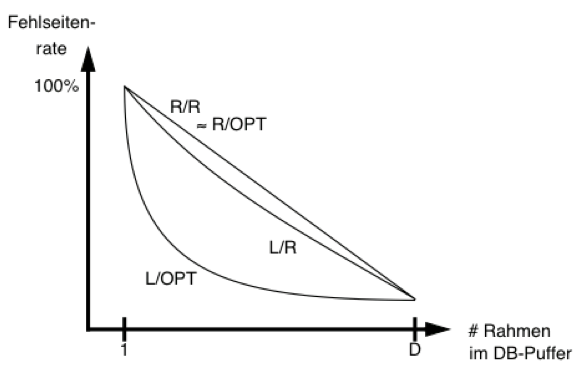
\includegraphics[width = 8cm]{Pictures/Ue07_Aufgabe2_Zusatz1.png}
\end{minipage}

\begin{tabular}{|l|l|l|l|l|}
	\hline
	 					& R/R 			& R/OPT 		& L/R 			& L/OPT 		\\
	\hline
	Referenzen 	& Random 	& Random 	& Lokalität 	& Lokalität 	\\
	\hline
	Ersetzung 	& Random 	& Opt 			& Random 	& Opt 			\\
	\hline
\end{tabular}

Belady-Optimal: Ersetze die Seite, die am längsten in die Zukunft nicht referenziert wird.